\chapter{Missing Transverse Energy reconstruction and correction}
Atlas detector has almost 4$\pi$ coverage. This is allowing to calculate imbalance of energies inside calorimeter, especially transversal part of it called \etmiss.  Neutrino from a $W \to l\nu$ decay is leaving detector, without interacting with it, that is causing large energy imbalance in a detector. 

Standard reconstruction of \etmiss at \atlas experiment uses transverse energy deposits in the calorimeter, energy losses in cryostat and reconstructed muons for a calculation:
\begin{equation}
E_{x(y)}^{miss} = E_{x(y)}^{miss, calo} +  E_{x(y)}^{miss, cryo} +  E_{x(y)}^{miss, muon}.
\end{equation}
Calorimeter term is using information from reconstructed physics objects for calibration of cell responce. The total transverse energy in calorimeter is defined as:
\begin{equation}
E_{x(y)}^{miss} = E_{x(y)}^{miss, e} + E_{x(y)}^{miss \gamma} + E_{x(y)}^{miss, \tau} + E_{x(y)}^{miss, jets} + E_{x(y)}^{miss,SoftTerm} + E_{x(y)}^{miss, \mu}.
\end{equation}
where each term is calculated as the negative sum of the calibrated reconstructed objects, projected onto the x and y directions. Each jet with energy $P_T$>20 GeV is corrected for a pile-up and a jet energy scale is applied. Soft term is calculated from topoclusters and tracks, that are not assosiated with high-pt objects. To avoid double counting muon energy loss is in calorimeter is  subtracted from \etmiss.  The \etmiss muon term is calculated from the momenta of muons measured in a range of pseudorapidity. Since pileup gives a significant effect on a \etmiss performance several methods of pileup suppression are used
\begin{figure}[b]
\begin{minipage}[h]{0.49\linewidth}
\center{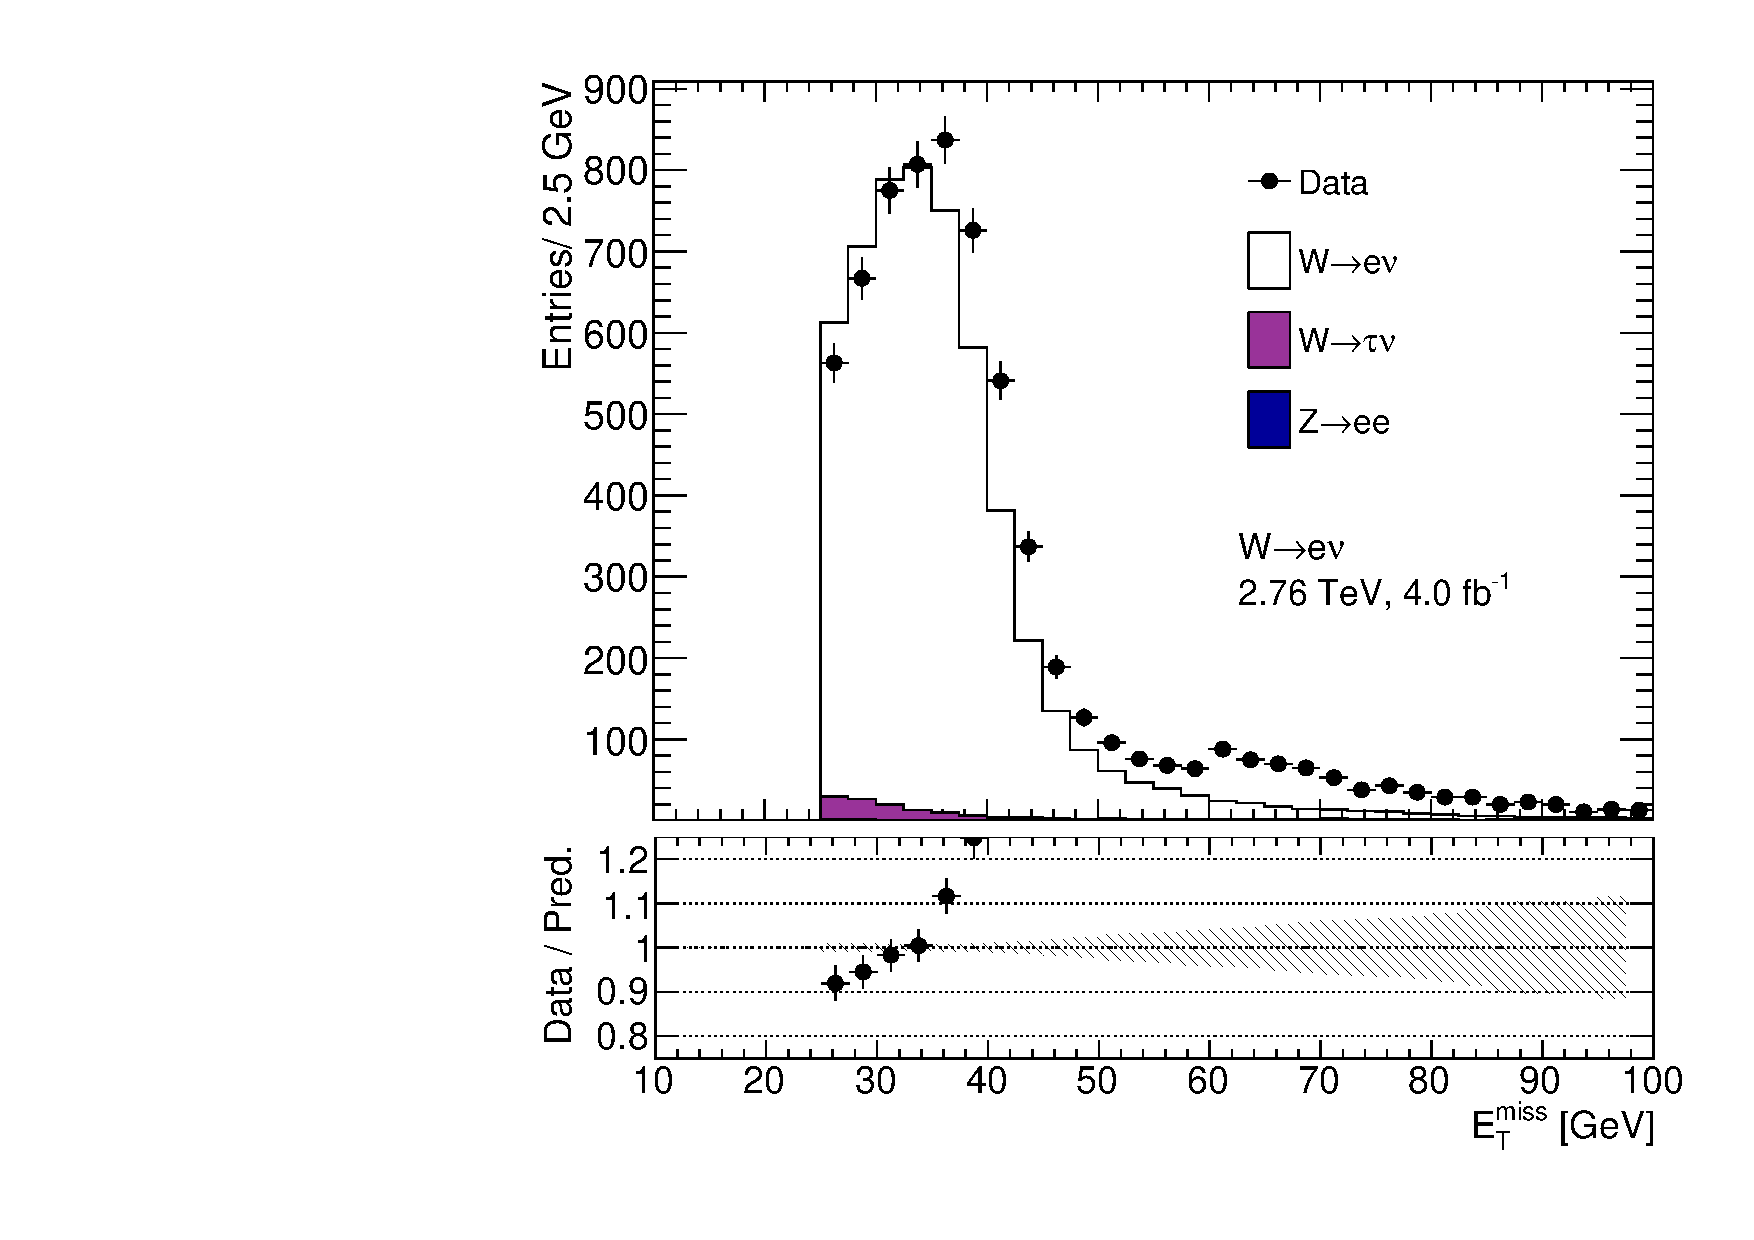
\includegraphics[width=1.\linewidth]{HadronRecoil/WenuRefFinal.pdf} \\ a)}
\end{minipage}
\hfill
\begin{minipage}[h]{0.49\linewidth}
\center{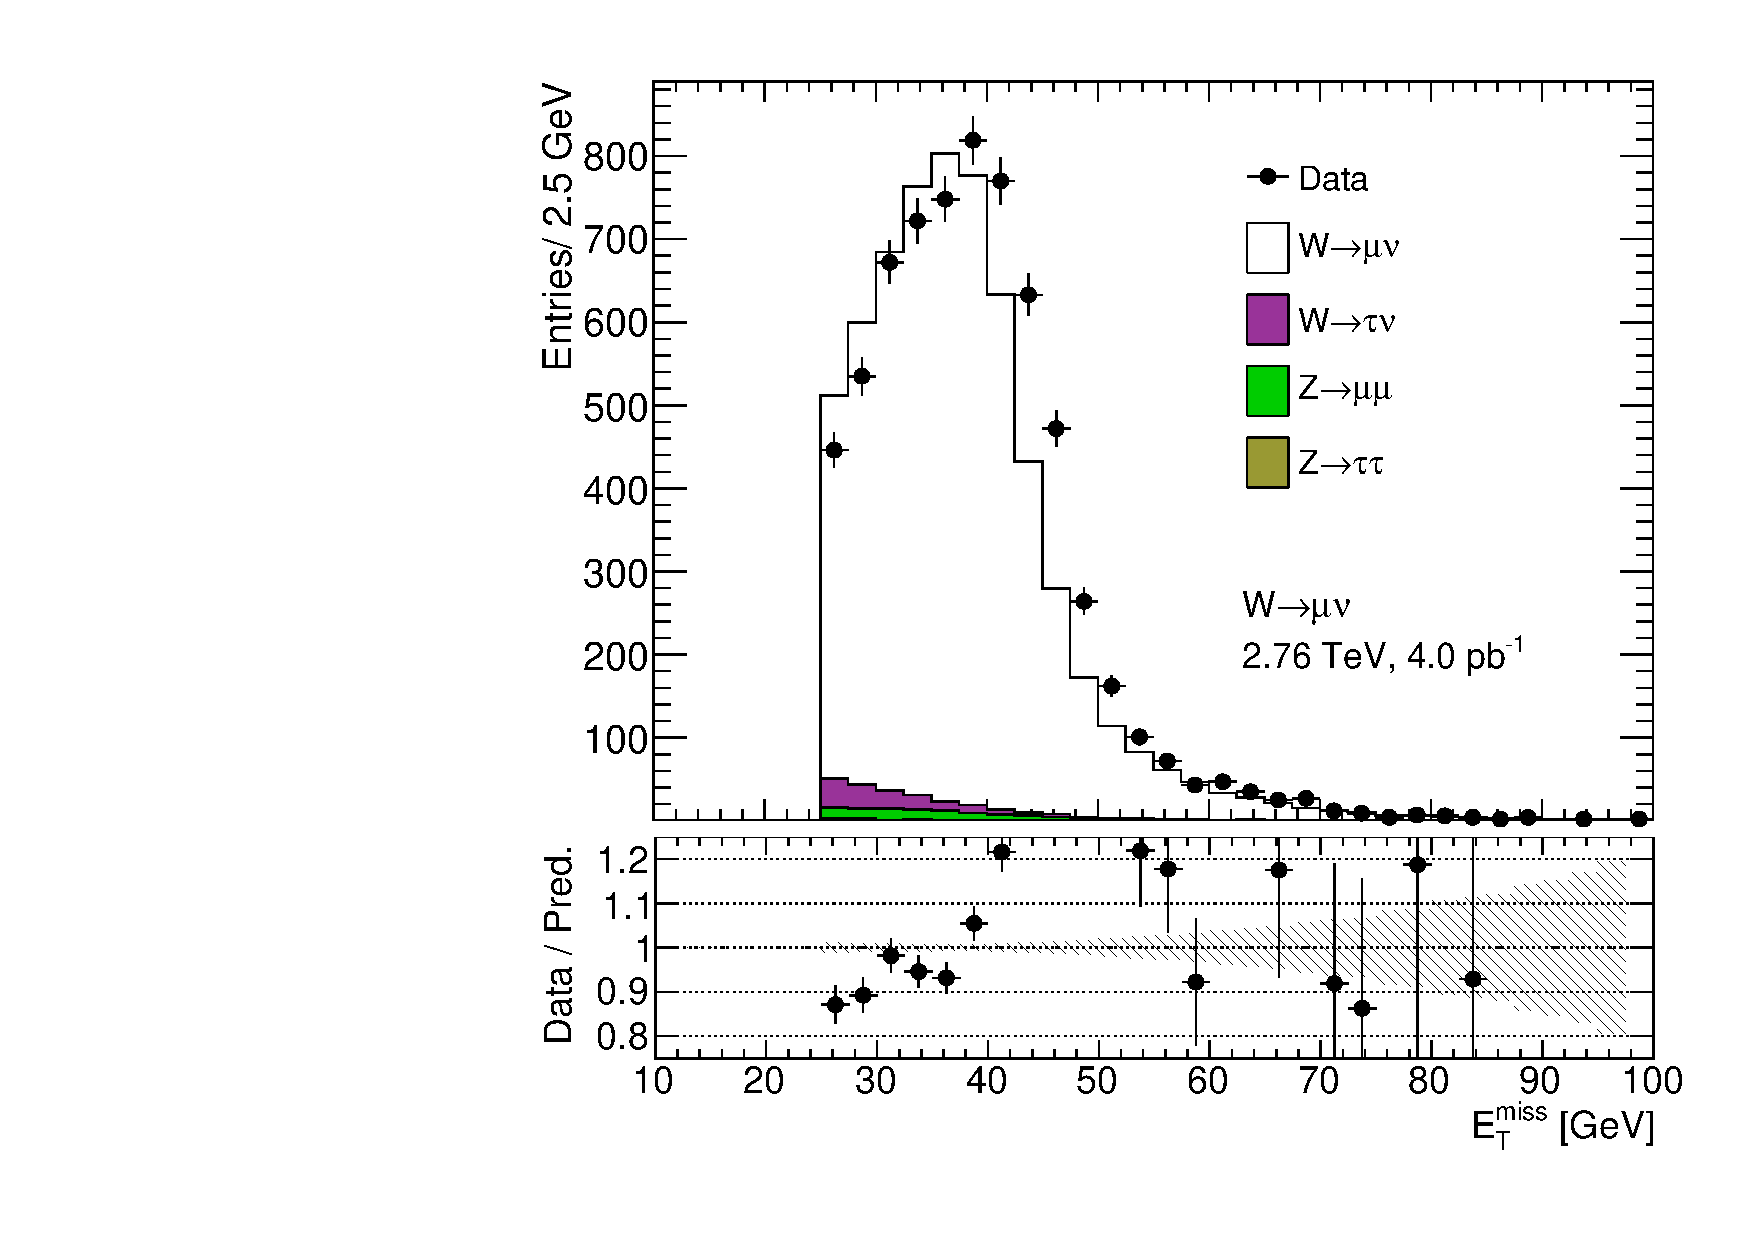
\includegraphics[width=1.\linewidth]{HadronRecoil/WmunuRefFinal.pdf} \\ b)}
\end{minipage}
\caption{Data and MC comparison for \etmiss calculated by standard \atlas algorithm for a)\wenu b)\wmunu events}
\label{ris:EtMissRefFinal}
\end{figure}
This procedure was optimised for 8 TeV runs  and using a calibration constants from it. This can cause problems with 2.76 TeV low pileup run. As a examine showed this is not optimal procedure in this case. Control plots for W production in electron and muon channels are shown on a  Fig. \ref{ris:EtMissRefFinal}. Where a big discrepancies in a muon and electron channel, that cannot be accounted to multijet background. 

\begin{figure}[t]
\begin{center}
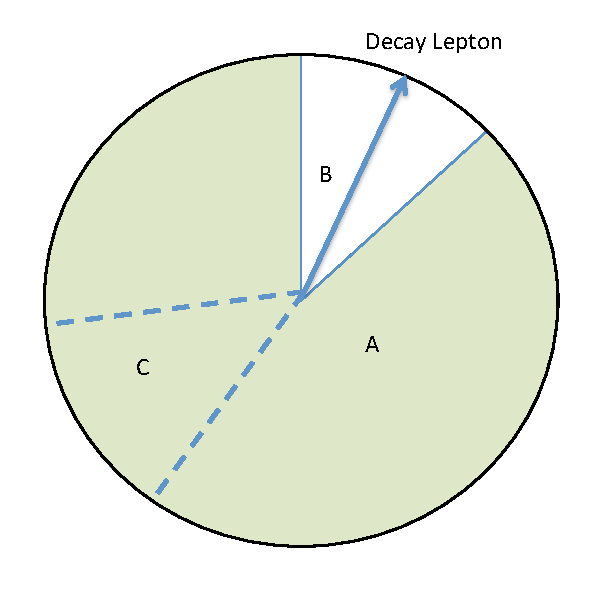
\includegraphics[width=0.6\textwidth]{HadronRecoil/ReplacementCluster.pdf}
\caption{Definition of different zones in the calculation of the cluster-based hadronic recoil. \label{ris:subsCone}}
\end{center}
\end{figure}


\section{Hadron Recoil Calculation}
Second way of calculating \etmiss was developed specifically for a W and Z decays by W mass measurements group. This procedure is using this fact, that a transverse momentum of a W-boson has to be balanced with initial (quark-gluon) state radiation, because initial sum of transverse momentum is zero:
\begin{equation}
\vec{P_{T}^{W}} = \vec{P_T^{lep}}+\vec{P_T^{\nu}}= \sum{\vec{P_{T}^{ISRquarks,gluon}}}, 
\end{equation}
where $\sum{\vec{P_{T}^{ISRquarks,gluon}}}$ is a transverse momentum of partons from initial state radiation, also called hadronic recoil (HR). Therefore, \etmiss can be determined as:
\begin{equation}
E_{T}^{miss} = P_T^{\nu} =  - HR + p_T^{l}
\end{equation} 

This procedure assumes, that recoil is arises from one single leading jet, and the rest  is coming from a soft hadronic activity. This hadron recoil is computed as a vector sum of calorimeter clusters:
\begin{equation}
HR= \sum_{i=0}^{N_{topo}}\vec{p_T^{topo}}
\end{equation}
while a scalar sum of all transverse energies is corresponding to the hadronic activity of the event:
\begin{equation}\label{eq:sumet}
\sum E_T =\sum_{i=0}^{N_{topo}} E_T^{topo}
\end{equation}
To avoid double counting of lepton energy losses in calorimeter, the clusters inside cone with radius dR = 0.2 are excluded from this calculation.To compensate soft activity inside this cone, clusters are then compensated by replacement cone (Fig. \ref{ris:subsCone}). This cone is defined as cone at the same pesudorapidity, but different $\phi$. It should be far from any other lepton and hadron recoil direction. Each cone is then rotated to a direction of the original lepton direction. This definition is not taking into account jet reconstruction aspects.   This is allowing to get a better data MC agreement (Fig. \ref{ris:HadrRecoilEtMiss}).
\begin{figure}[b]
\begin{minipage}[h]{0.49\linewidth}
\center{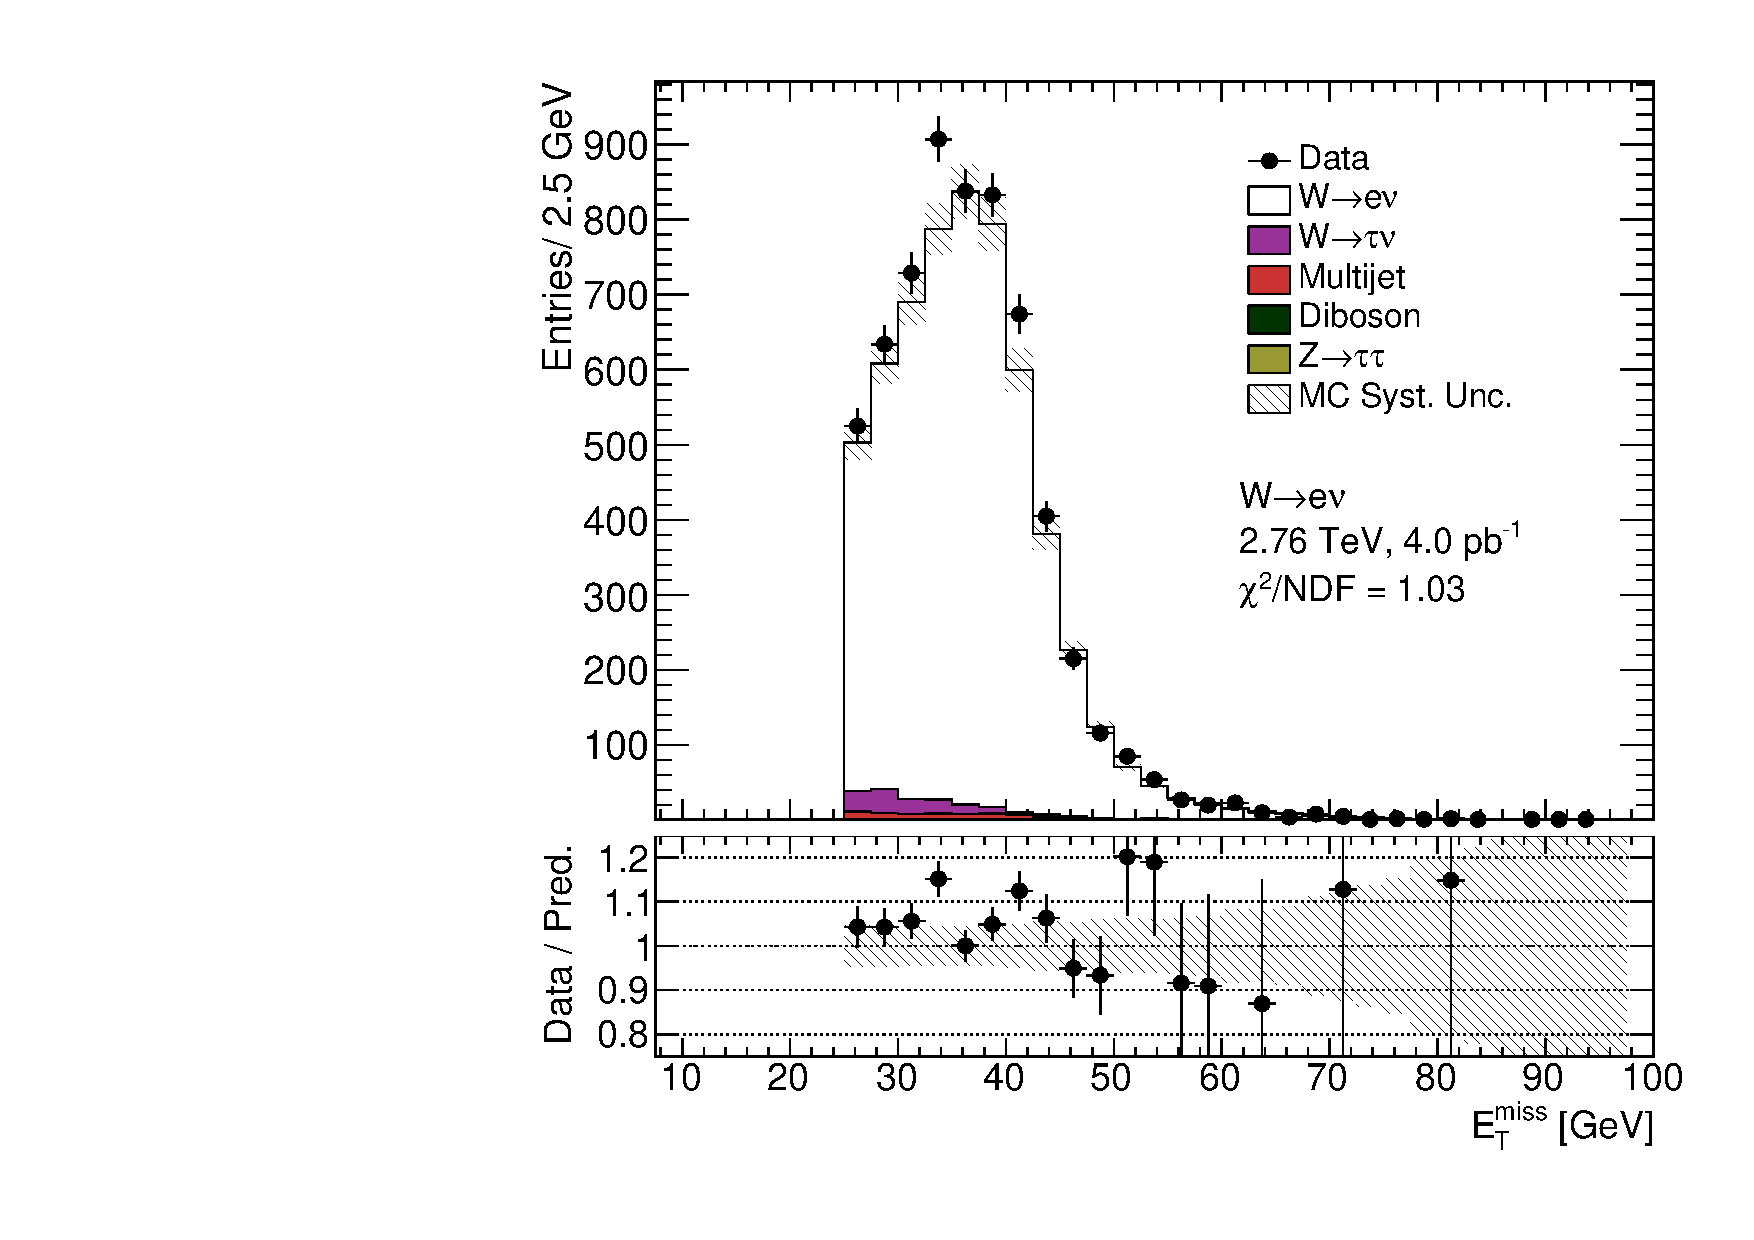
\includegraphics[width=1.\linewidth]{HadronRecoil/W_Boson_etMiss.pdf} \\ a)}
\end{minipage}
\hfill
\begin{minipage}[h]{0.49\linewidth}
\center{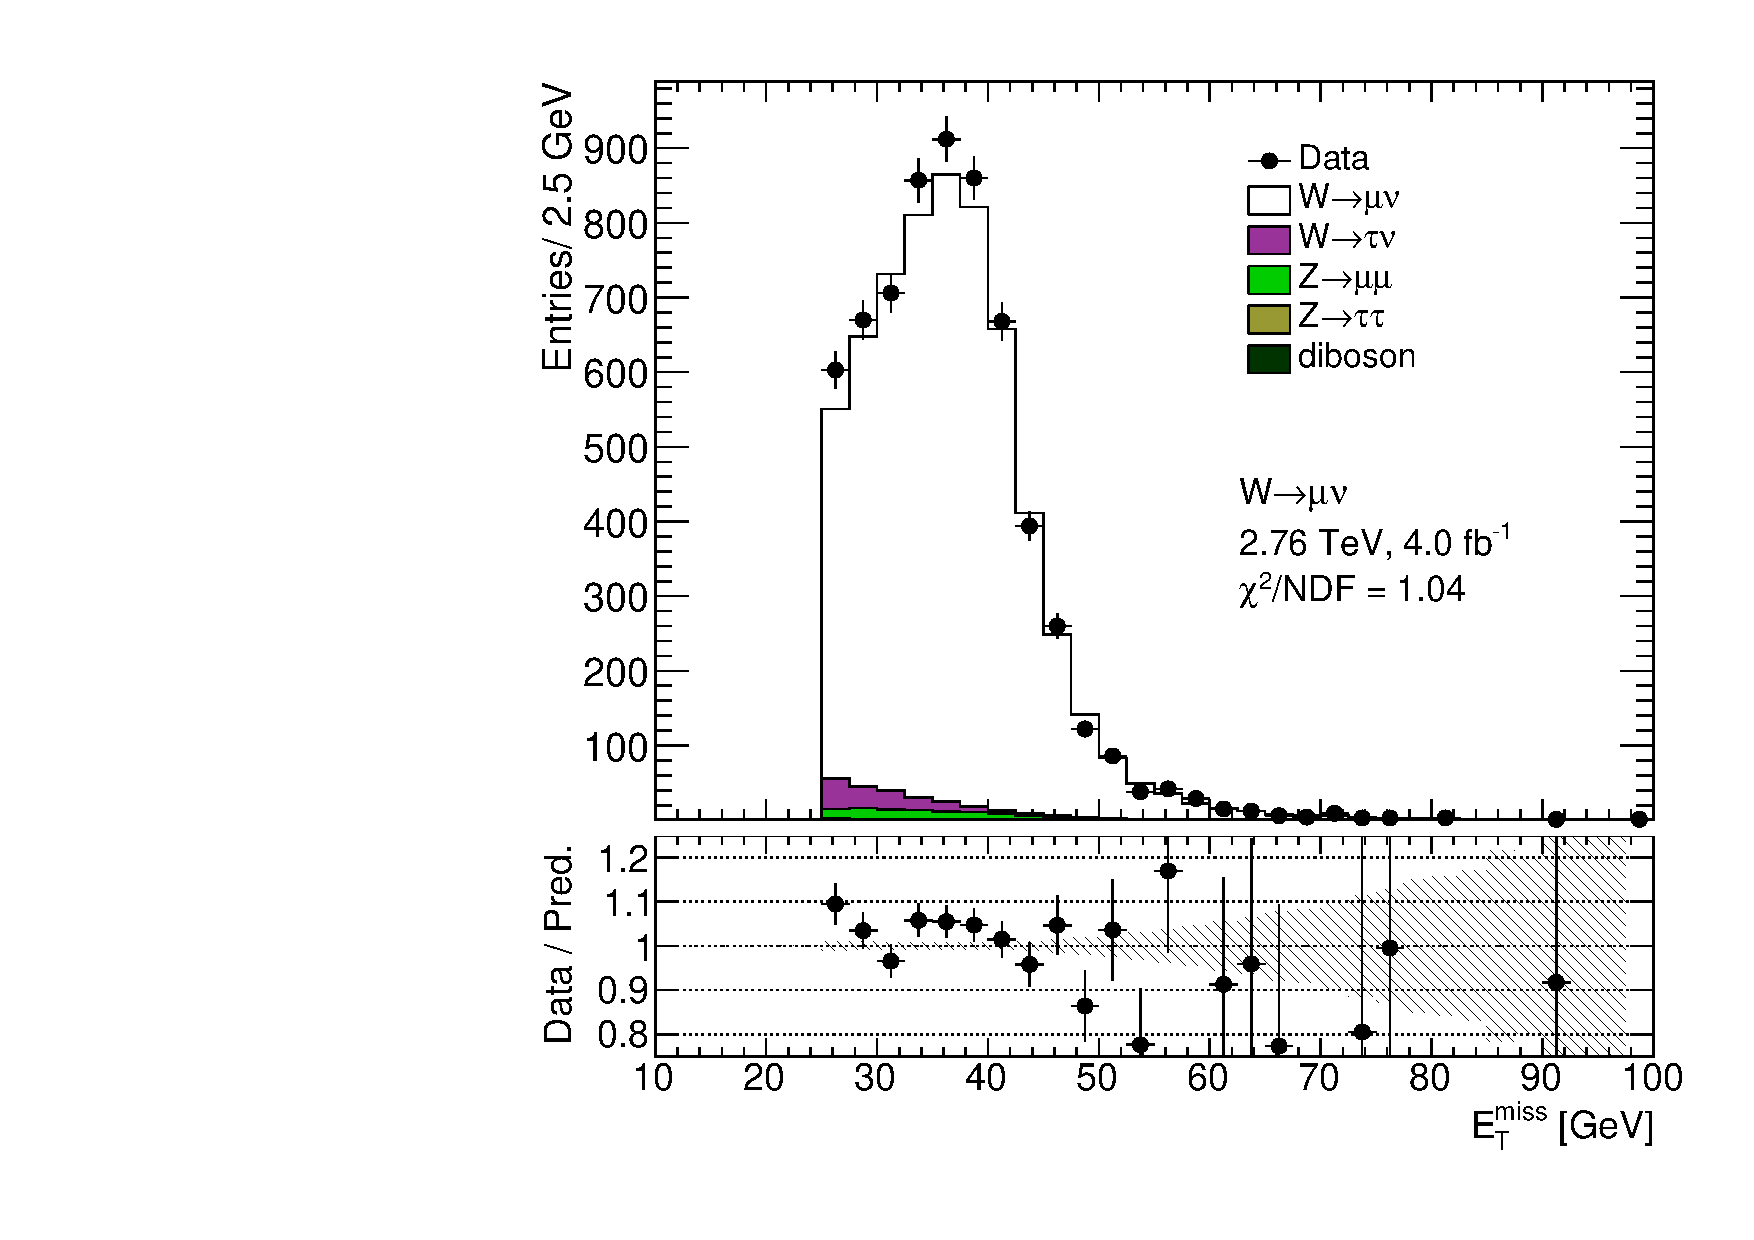
\includegraphics[width=1.\linewidth]{HadronRecoil/Wmu_Boson_etMiss.pdf} \\ b)}
\end{minipage}
\caption{Data and MC comparison for \etmiss calculated from hadron recoil for a)\wenu b)\wmunu events}
\label{ris:EtMissRefFinal}
\end{figure}



where $\vec{v}$ is the unit vector along boson $p_{T}$ direction. Parallel component is sensitive to a bias relative to a truth \pt of the boson, while perpendicular component is 0 on average and affected just by a resolution effects.  
Momentum of Z boson can be preciselly determined by a measurement of its decay products. This is allowing to determine data driven hadron recoil corrections. Due to a low cross-section of Z production, this corrections are mostly statistically dominated.
On another hand, it is also possible to use W boson decays for a not so systematicslly precise, but statistically better. 

However, due to a limited statistics of a Z decays in this data, it is better to combine this with a corrections derived from W decays da

\begin{figure}[t]
\begin{center}
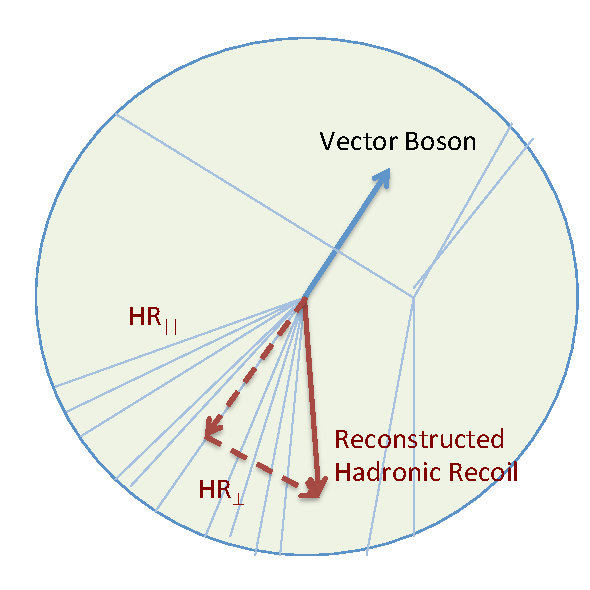
\includegraphics[width=0.6\textwidth]{HadronRecoil/RecoHRParPerp.pdf}
\caption{Parallel and perpendicular projection of the hadronic recoil with the respect to the transverse momentum of the vector boson \label{ris:HadrRecoilTruthPt}}
\end{center}
\end{figure}

\section{Hadron Recoil calibration}
\etmiss affects significantly on a W boson measurement, so its important to have good understanding of sources of a possible differences in a hadron recoil reconstruction in a data and monte carlo. 

This differences can be paramerised at the respect of the truth boson Pt as follows:
\begin{equation}
,
\end{equation}
where \upar is a projection to the direction of the truth boson pt, and \uperp is the projection on a perpendicular plane. On average \upar should be match absolute value of boson pt and thus this quantity is sensitive to a relative bias of hadron recoil reconstruction. On another hand \uperp comes from calorimeter resolution and should have 0 mean. This component is sensitive to a discrepancies in data/mc resolutions. 
Standard procedure of calibrating hadron recoil uses Z boson, since its transverse momentum can be determined not only by a hadron recoil, but also from its decay products.  Zpt resolution coming from lepton reconstruction is around 10 GeV, while hadron recoi resolution is around 30 GeV, what is alowing to have a precise determination of a calibration constants. On another hand, size of the Z sample in 2.76 TeV data is small, so this constants will be statistically dominated.
On another hand, in W decays hadron recoil corrections cannot be determined through boson pt directly, but this channel has a better statistics.  The  procedure is more complicated, because it should not change truth boson spectrum and not correct additionally boson pt mismodelling.
At the end, the combination of 2 determination results have been used. This section describes a procedure of calibrating bias and resolution mismodelling in a hadron recoil, that was apapted for 2.76 TeV data. 

\subsection{Underlying event mismodelling correction}
One of the possible sources of diffetences in data and MC is a modelling of underlying event. Soft interactions cannot be computed precisely by a pertrubative quantum chromodynamics methods, so it is usually described by a phenomenological models, that can be not so precise.  
Pile-up mismodelling usually accounted by correcting average number of interaction per bunch crossing to match a data. However, \atlas simulation is suited for an ordinary high pile-up runs, so this quantity is not modelled well in a case of 2.76 TeV analysis \ref{ris:Mu.png}. 

Another quantity that depends on a underlying event is a \sumet, defined in a Eq. \ref{eq:sumet}.   There is a visible shift between data and monte carlo in a both channels. This is causing differences in a hadron recoil resolution, since this variables are highly correlated (add some figure).  Size of the Z sample is not sufficient to determine the correction factors, so the W boson was used. 

To leave boson pt spectrum untouched, correction factors are determined inside pt bins as:
\begin{equation}
SF^{channel}=\frac{\sum E_T^{data} (p_T^{W, rec})}{\sum E_T^{MC, channel} (p_T^{W, rec})},
\end{equation}
where $\sum E_T^{data} (p_T^{W, rec})$ and $\sum E_T^{MC, channel} (p_T^{W, rec})$  are a \sumet distributions inside $p_T^{W, rec}$ for data and monte carlo respectively. Scale factors are determined separatelly for each signal process.  In order to increase statistics in data the combination of \wenu and \wmunu processes is used. Example of this correction factors for \wPlusenu is shown on a Fig. \ref{SFWplusenu}. 

The distribution of \sumet after correction is shown on a Fig. \ref{sumetAfter}. Reconstructed and truth boson spectrum is staying untouched (Fig. ).  Systematic error coming from this method can be studied by parametrisation  of scale factors with polynomial order 2 inside each $p_T^{W, rec}$ bin.  
Statistical uncertainty correction can be determined through the uncertainties of this approximations. Set of the scale factors with polynomial parametrisation have been produced. For each scale factor inside this set polinomial parameters have been varied inside its unsertanty (correlation between parameters have been taken into accound). 
Systematical errors can be determined by using additional parametrisation of scale factor inside the bin with polynomial. 
The overall effect on a \cw for a different methods is shown in a Tab. \ref{SumetCW}.  As it can be seen, sign of the effect is different for electron and muon flavor of the analysis. 
 


\subsection{Hadron recoil bias correction}


As it was mentioned before, it is possible to use both Z and W boson sample for hadron recoil bias determination. Correction factor $SF_{HR,bias}$ is applied as:
\begin{equation}
\upar^{MC,cor}=\upar^{MC} \cdot SF_{HR,bias},
\end{equation}
and can be obtained by scanning the impact of the scaling factor on the Data to MC agreement of the distributions that are dominated by the recoil scale uncertainties. Since W boson has no second source of \ptw measurments, determination of the hadron recoil bias should use the distributions, that  are not sensitive to a truth \ptw spectrum.  One of the optimal choises is a \mtw distribution. Transverse mass distribution for a different scale choises is shown on a Fig. \ref{HadronRecoilScaleMtW}. Multijet background is not included, because it shape and number of events is depending on a hadron recoil scale and thus can introduce additional systematics.
The first way to determine correction factor is using a difference in the mean of transverse mass in data and MC. Statistical error of this determination is an error of the mean in the data. The precision of this method is low, is it is mainly used as a cross-check. 
Second way is calculating \chi2 for each correction factor. The ideal correction factor is determined by fitting \chi2 distribution by the function:
\begin{equation}
\chi2 = \frac{(x-sf_{best})^2}{\sigma_{sf}^2}+\chi^2_0,
\end{equation}
where $sf_{best}$ is the best scale factor and $\sigma_{sf}$ is a statistical error of this parameter. Distribution of \chi2 and a fit in combined W channel is shown on a Fig. \ref{mtWChi2}.
Because of the possible mismodelling of the tail \mtw distribution it is not included in a \chi2 calculation, leaving a free choise of the parameter of the cutoff.  It is also possible to exclude regions with high multijet background contamination by applying a tighter cut on a \mtw. This fit range is introducing one source of systematic error. Effect of the range on value determination is shown on a Fig. \ref{ScaleMtWRange}. Similarly to a W channel, scale correction in a Z sample can be determined from distribution $\frac{\upar}{\p_T^{ll}}$, shown on a Fig. \ref{uPAr}. Since there is no choise of the range and dependency on $P_T^{bos}$ modelling, there is just one source of uncertainty.  
Results on a hadron scale factros and it's errors are shown in a Table \ref{tab:SFHadronRecoil}. The results are consistent within 1 sigma. Overall effect on a Cw is shown on a Tab. ~\ref{tab:CWHadronRecoilScale}.


\subsection{Hadron recoil resolution correction}

